
\chapter{Methods}

%intro
%TCSPC technique
%problemi ed errori
%simulazioni e cose da tenere presente

\section{Time Correlated Single Photon couting}

The time correlated single photon couting (TCSPC) technique, makes use of low-level signals at high repetition rate, with the probability of detecting on photon in one repetition period being very low \cite{Becker2005}.
It is then sufficient, to determine the time profile of the sample, to measure the time of arrival of single photons and build up a histogram of the photon times.
The most common method to perform this measurement is a start-stop setup: some sort of trigger, correlated with the beginning of the exctitation process in the sample (start), is measured in coincidence with a stop signal given by the arrival of the optical photon emitted by the sample.
\begin{figure}[htbp]
\begin{center}
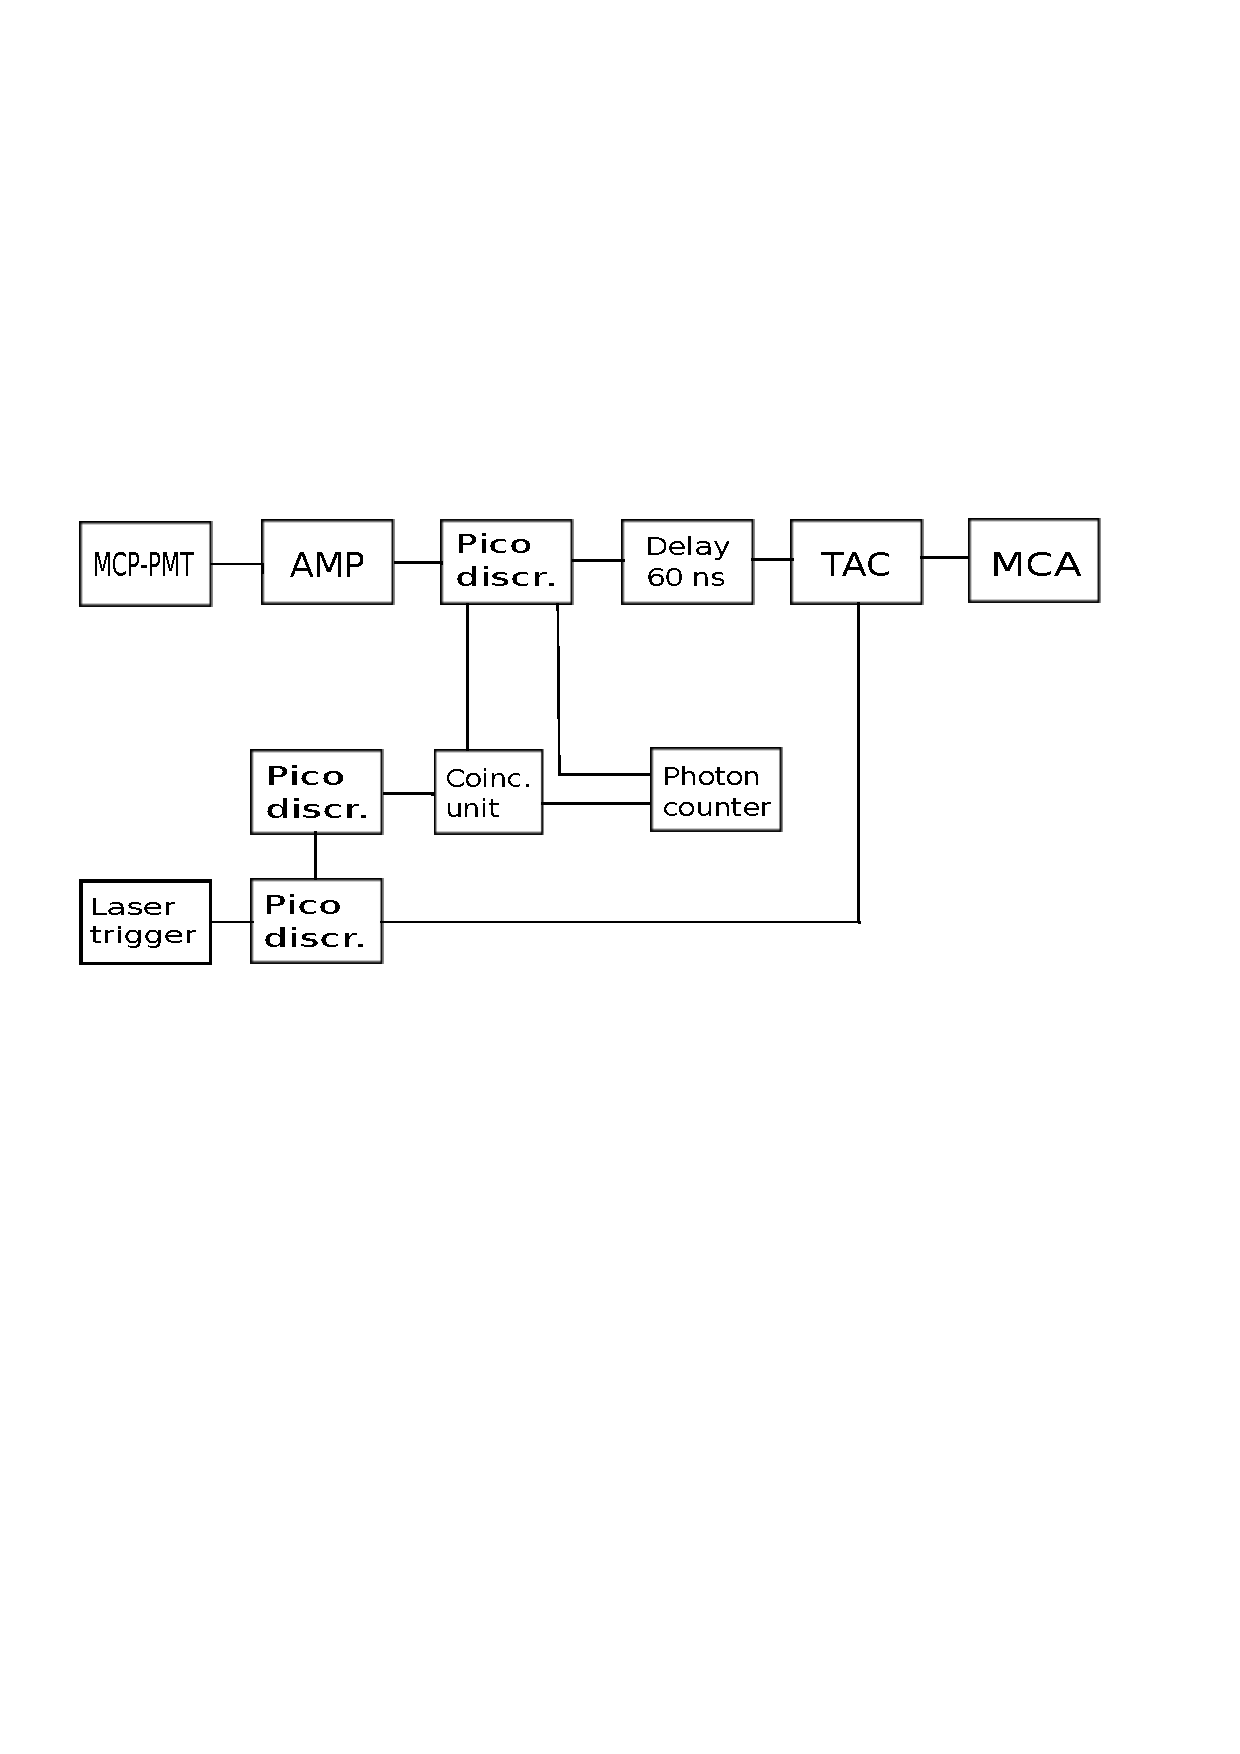
\includegraphics[width=9cm]{../Pictures/Chapter_8/electronics.pdf}
\end{center}
\caption[TCSPC technique]{Principles of time correlated single photon counting (TCSPC)}
\label{fig:daw}
\end{figure}
Thus the main components of a TCPSC system are
\begin{itemize}
\item an excitation system for the sample with an extracted trigger
\item a fluorescent sample with a characteristics periodic light emission
\item a detection system able to extract the time stamps of the arriving single photons.
\end{itemize}
The effective resolution of a TCSPC experiment is characterised by its instrument response function (IRF). The IRF contains the pulse shape of the light source used, the temporal dispersion in the optical system, the transit time spread in the detector, and the timing jitter in the recording electronics.
The main sources of error and incertitude on the measured curve are presented in this chapter and can be roughly cathegorized as:
\begin{itemize}
\item the time structure of the excitation
\item the single photon time resolution of the detection system
\item the rate of arrival of optical photons at the stop detector
\item the accumulation times: statistics
\end{itemize}

\subsection{Excitation}
In an ideal TCSPC experiment, the excitation system has a very narrow distribution in time. That is, the spread of the single particles determining the excitation of the sample is negligible with respect to the time scale of the processes under study.
A variety of high time resolution sources are available for TCSPC. In classical fluorescence studies laser sources (or laser-driven) sources are used and allow for the study of sub-ps dynamics: mode-locked Argon or Nd:YAG lasers, synchronously pumped dye lasers, or Ti:sapphire laser.
For the time scales that characterize electron hole thermalization, thus signal formation, thus rise time in scintillating crystals, it is necessary to make use of a ps resolved system.

The main limitation though, comes from the excitation energy of the system, since the level of excitation is crucial in determining the physical processes that concurr to give a non zero rise time. 
As was shown in previous chapter, the multi scattering processes that lead electrons and holes below the ionization threshold, and thus to the accuracy limit of Monte-Carlo simulations, happen on time scales which are an order of magnitude inferior to the thermalization stage. 
This means that in terms of physical processes not much is added to the study by raising the excitation energy above 10 time % check!!
the band gap of the sample.
Two different phenomena though introduce a non negligible contribution to the time spread of the rise if the signal collected.

The first one is the appareance of Cerenkov photons, above the threshold for the specific materials. Thresholds for Cerenkov effect in heavy scintillating crystals have been briefly summarized in chapter %specificare tabella.
As will be diffusely discussed in %dove lo discuti
this photons, though in a limited number, are concentrated in the very first portion of the time profile. This results in a modification of the rise time towards longer values.
In order to disentagle this variety of effect, the sample were measured in different conditions of excitation: at a high harmonics generation facility with a 36 eV VUV radiation and in a experimental bench with a 511 KeV radiation.

A second prominent source of smearing in time profiles is the travel of photon inside crystalline samples \cite{Derenzo2000}. Indeed, depending on the type of coupling to the photo detector, photo extraction can be favoured or disfavoured at different angles. Opening this extraction cone accounts for different time profiles: a Teflon diffusive wrapping or coating for example, gives longer rise times. From the point of view of the excitation energy, though, an important difference can be found at 36 eV or 511 KeV. In the first case the excitation is only on the surface, since the range of VUV photons in a heavy scintillator is
% metti il range 
In the case of excitation at higher energy, on the other hand, photons may travel longer distances in the lattice, and photons produced in the deep volume of the sample need to be coupled out.

\subsection{Detection}

Once the sample has been excited, photons are couple out to the stop detector. Tipically PMTs, MCP-PMTs or single cell APD in Geiger mode are the preferred detectors for their timing characteristics. The crucial parameter in this case is Single Photon Time Resolution (SPTR) for Silicon detectors or Transit Time Spread (TTS) for vacuum detectors.
% sptr TTS
When a photocathode is fully illuminated, the transit time of each photoelectron pulse has a fluctuation. This fluctuation is called TTS (transit time spread).
It is clear that in order to extract the most accurate value for the time constants of the samples measured, one should keep the incertitude component due to the detector as low as possible. In this case though, it is customary to make use of detectors optimized for single photon detection, that is with low or no energy resolution and very rapid response.
For the study presented MCP-PMTs have been mainly used, since in principle they guarantee the best performance when considering acquisition rates and time resolution.
As will be clear in the next chapters, this prerogative of MCPs becomes less and less attractive as the energy of the excitation grows, since it is necessary to cope with non negligible backgrounds due to the high active area.
Nevertheless, given the time scale considered in this study, a response of less than 100 ps should be available in order to extract the parameters with a minimum accuracy. As will be presented in the next chapters the photo detectors chosen for this study satisfy this requirement.
Many stop detectors, and this is the case of the MCPs used in the next analysis, present important amount of time walk, and often require appropriate corrections.
Time walk arises when synchronous signals have different amplitudes. Time pick up methods based on threshold crossing may extract different time stamps and thus introduce a non negligible jitter, as shown in figure \ref{fig:}.
%qua ci vuole una foto del time walk, yes on the time walk. Too sexy for Milan, New York and Japan

\subsection{Stop rate and bias}
When considering the geometry of the experiment, another parameter becomes crucial, the stop rate at the detector.
As explained before two opposite effects tend to counteract; ideally we should keep the count rate as high as possible to have reasonable accumulation times, but the increasing of the bias fraction of counts modify the profile measured.
Two techniques will be used in this study, employing a conventional TDC and a multi-hit TDC.
A conventional TDC can only digitize the arrival time of the first stop signal. Therefore events that have more than one stop pulse will bias the dataset, since the later pulses will not be measured with the same probability. This will be the case of the acquistion setup presented in chapter 7.
If we define the probability P that m photons are detected after a single excitation, the Poisson distribution gives
\begin{equation}
P(m;\epsilon) = \epsilon ^{m} e ^{-\epsilon} / m!
\end{equation}
and $\epsilon$ is the average number of stop per excitation.
The probability to have an unbiased event is
\begin{equation}
Event_{unbias} = U = P(1;\epsilon) = \epsilon e ^{-\epsilon}
\end{equation}
and the probability to have a biased event is, assuming $\epsilon << 1$
\begin{equation}
Event_{bias} = B = \sum _{m = 2} ^{\infty} P(m;\epsilon) \sim \epsilon ^{2} e ^{-\epsilon} / 2
\end{equation}
The ratio of biased to unbiased event is given by
\begin{equation}
$B/U \sim \epsilon / 2$
\end{equation}
The factor $\epsilon$ depends on the combined effect of the geometry of the system, the light yield of the crystal, the quantum efficiency of the detector. In order to improve the ratio, it is thus necessary to lower the rate at the detector by modyfing the position accoridngly, at the expense of reduced data collection rates.

On the other hand, in chapter 8 a multi hit approach will be proposed, that is capable of measuring the arrival if n stop pulses per start pulse. In this configuration the data acquisition rate can be increased, as the probability is:
\begin{equation}
Event_{unbias} = \sum _{m = 1}^{n}mP(m;e) = \sum _{m = 1}^{n} \frac{\epsilon ^{m}e^{-\epsilon}}{(m-1)!}nj
\end{equation}
In particular dead casad
% rapidamente i due parametri che ci interessano

% come abbiamo scelto la bias fraction

% immagine con troppo bias?

% e poi le due il decay fatto per diversi delta

% e poi spiegare che il rise e' meno drammatico, calcolato quindi per un solo valore, che poi e' il nostro grafico

%\subsection{Statistics and accumulation times}

% questo lo voglio fare? cé da capire la vicenda della varianza!

\section{Data analysis techniques}
In order to analize the start stop data collected, a classical fitting approach was used, based on maximum likelihhod principles.
With respect to this statistical and sistematic contibution to the error were estimated, based on the previous discussion.
In particular the iterative reconvolution approach has been used, being the most powerful and widespread in the field of fluorescence lifetime measurements.

\subsection{Iterative reconvolution}
In time correlated single photon counting experiments the problem at hand is statistically speaking to estimate or more parameters (the lifetimes) from a dataset.

The maximum likelihood method is considered to be the most powerful method of parameter estimation.
Consider $n$ independents observation (counts in this case) c$_{1}$, ... , c$_{n}$ and a vector of parameters \textbf{$\theta$} = $(\theta _{1},...\theta _{m})$. If the probability of having the observation i is $p(c_{i}|\theta)$, the likelihood function is
\begin{equation}
L(c_{1},...c_{n}|\theta) = \prod _{i = 1} ^{n} p(c_{i}|\theta) 
\end{equation}
The Maximum Likelihood method provides then an estimate of the true parameters' value as the vector \textbf{$\theta$} that maximizes the likelihood function.
In the case of time correlated single photon counting it is natural to assume that the observed counts $c_{i}$ follow a Poisson distribution
\begin{equation}
p(c_{i}|\theta) = \exp{ \left( -<c_{i}>\right) }\frac{<c_{i}>^{c_{i}}}{c_{i}!}
\end{equation}
where $<c_{i}>$ is the expected value of the number of counts in the i-channel.
This expected value is given by the model taken in to consideration: in this case we can make use of the equations optained in chapter 3. The pdf for the time stamps is given by
\begin{equation}
p_{t_{n}}(t|\theta) = A \cdot \sum _{i} \frac{S_{i}}{\tau _{d,i} - \tau _{r,i}} \cdot \left[ a_{\tau _{d, i}}(t|\theta) - a_{\tau _{r,i}}(t|\theta)\right]
\end{equation}
where 
\begin{eqnarray}
a _{\tau}(t|\theta) &=& \frac{1}{2} \exp{\left(\frac{\sigma _{SPTR} ^{2} - 2t\tau +2\theta \tau + 2t_{TT}\tau}{2\tau ^{2}}\right)} \\
&& \cdot \left[ erf\left( \frac{t-\theta -t_{TT} - \frac{\sigma ^{2}_{SPTR}}{\tau}}{\sigma _{SPTR}\sqrt{2}} \right) + erf \left( \frac{t_{TT}+\frac{\sigma ^{2} _{SPTR}}{\tau}}{\sigma _{SPTR}\sqrt{2}} \right) \right]
\end{eqnarray}
Thus the expected number of counts for the i-channel is
\begin{equation}
<c_{i}> = \int _{(i-1)\Delta} ^{i\Delta} p_{t_{n}}(t|\theta)dt + b_{i} = g _{i}(\theta)
\end{equation}
where $\Delta$ is the time channel width and $b_{i}$ accounts for the average number of dark counts in the channel i.
The vector of parameters \textbf{$\theta$} is given by the lifetimes $\tau _{i}$, the relative intensities $S_{i}$ and a zero time shift $\delta$.
It is customary to determine the best estimate for \textbf{$\theta$} by minimizing the function $-ln(L)$ since the log-likelihood function attains its maximum for the same value as the likelihood function.
In the specific case the function to minimize is
\begin{equation}
-Ln(L) = - \prod _{i=1}^{n} \exp{-g_{i}} \frac{g_{i}^{c_i}}{c_{i}!} = \sum _{i=1}^{n} -g_{i} + c_{i}ln(g_{i}) - ln(c_{i}!)
\end{equation}
which is equivalent to minimizing the Poisson deviance\cite{Bajzer1991}
\begin{equation}
f = \sum _{i=1}^{n} -g_{i} + c_{i}ln(g_{i})
\end{equation}
The standard function minimized in standard fluorescence analysis is usually the $\chi ^{2}$ defined as
\begin{equation}
\chi ^{2} = \sum _{i=1}^{n} \frac{\left[ c_{i} - g_{i}(\theta) \right] ^{2}}{c_{i}}
\end{equation}
or, in the modified least square method\cite{Bajzer1991}
\begin{equation}
\chi _{m}^{2} = \sum _{i=1}^{n} \frac{\left[ c_{i} - g_{i}(\theta) \right] ^{2}}{g_{i}}
\end{equation}
When the number of counts is large they are numerically very close, since the Poisson distribution can be approximated by the Gaussian. Nevertheless in the data analysis the maximum likelihood estimator will be used, since it is preferable the more the low-count region of the decay influences the estimated parameters\cite{Bajzer1991}. 

\subsection{Sources of error}

%% qui il bias
%

%\begin{equation}
%P(m;\epsilon)P(any < DT) = \frac{\epsilon ^{m} e^{-\epsilon}}{m!}(1-exp(-(\frac{m!\delta}{2(m-2)!})))
%\end{equation}
%
%\begin{equation}
%P(m;\epsilon)P(none < DT) = \frac{\epsilon ^{m} e^{-\epsilon}}{m!}exp(-(\frac{m!\delta}{2(m-2)!}))
%\end{equation}
%
%\begin{equation}
%B/U = \frac{\sum _{2} ^{\infty} mP(m;\epsilon)P(any < DT)}{\sum _{1} ^{\infty} mP(m;\epsilon)P(none < DT)}
%\end{equation}


%\begin{equation}
%F_{hj} = \sum _{i}\frac{1}{y_{i}}\frac{\delta y_{i}}{\delta \alpha _{h}}\frac{\delta y_{i}}{\delta \alpha _{j}}
%\end{equation}
%
%\begin{equation}
%P(n, \alpha _{1}, \alpha _{2},...) = \frac{N!}{n_{1}!...n_{k}!} p_{1}^{n_{1}}\cdot ... \cdot p_{k}^{n_{k}}
%\end{equation}
%
%\begin{equation}
%(F^{multi})_{hj} = \sum _{i} \frac{1}{Np_{i}}\frac{\delta Np_{i}}{\delta \alpha _{h}}\frac{\delta Np_{i}}{\delta \alpha _{j}} = N\sum _{i}\frac{1}{p_{i}}\frac{\delta p_{i}}{\delta \alpha _{h}}\frac{\delta p_{i}}{\delta \alpha _{j}}
%\end{equation}
%
%\begin{equation}
%var_{N}(\tau) = (F^{m})^{-1}=\frac{1}{N}[F^{m}(N=1)]^{-1}
%\end{equation}
%
%\begin{equation}
%N > \frac{var_{1}(\tau)}{required variance (\tau)}
%\end{equation}
%
%%appendice sulla Poisson
%
%\begin{equation}
%p_{i} = \int _{\Delta T_{i}} f(t)dt
%\end{equation}
%
%\begin{equation}
%f(t, \tau , T) = \frac{1}{\tau} exp(-t/tau)\frac{1}{1-exp(-T/tau)} 
%\end{equation}
%
%\begin{equation}
%p_{i}(t, \tau, T) = \int _{(i-1)T/k} ^{iT/k} f(t, \tau, T)dt = frac{exp(\frac{T}{\tau k}) - 1}{1-exp(- t/\tau)} \cdot exp(-\frac{iT}{\tau k})
%\end{equation}
%
%\begin{equation}
%f(t, \tau _{R}, \tau _{D}, T) = [exp(-t/tau _{D}) - exp (-t/tau _{R})] \frac{1}{\tau _{R}[exp(-T\tau _{R})-1] - \tau _{D}[exp(-T\tau _{D})-1]}  
%\end{equation}
%
%


\section{Simulations}

\subsection{Study of optical transport}
\subsection{Cerenkov photons}